\section{Design and implementation}
\label{sect:design-and-implementation}

In this section we present \natisand, our proposal to enable the isolation
of native code for JS runtimes.

\subsection{Objectives}
\label{subsect:objectives}

We start with the definition of the design objectives.

\paragraph{Security}
As a secure sandbox, \natisand must provide protection against recent,
high-severity vulnerabilities affecting native components used by web
applications. Furthermore, the additional protection must not result
in a loss of functionality. The goal is to enable the developer to
follow the least privilege principle when designing its application,
reducing the attack surface in the presence of vulnerabilities.  To do
so, \natisand must be able to execute distinct native code in separate lightweight
compartments isolated from the rest of the application, and
characterized by policy-based ambient rights. The security
restrictions must be enforced independently of the method leveraged by
the application to execute native code, giving the developer the power
to confine executables, shared libraries, and functions. Lastly, no
root permission should be used at runtime to configure and activate
the isolated compartments.

\paragraph{Usability}
An important requirement to consider is usability by developers.  We
cannot force them to rewrite their application (or large parts of it)
just to use the sandbox. At the same time, we cannot expect them to be
aware of the internal structure of the third-party native code used by
the application, nor to fully understand the advanced security
mechanisms that can be leveraged to securely sandbox a program. The
effort required to take advantage of \natisand should be extremely
low. Ideally, a single configuration file specifying the ambient
rights associated with each compartment should be enough to
successfully configure it. To facilitate the transition from no
sandboxing to complete isolation, a valuable solution should permit to
start by sandboxing the components associated with the highest risk,
and then gradually extend the protection to the remainder of the
application.

\paragraph{Compatibility}
A valuable solution should be generic enough to be integrated into
different JS runtimes without requiring substantial changes to the
internal architecture. This also means that it must be aligned with
the current permission-based model implemented by the most widely used
platforms. Moreover, it must be compatible with other access control
mechanisms already enabled by the underlying OS. This refers to the
potential of stacking the sandbox on top of security mechanism adopted
by other software.

\paragraph{Performance}
Latency and throughput are critical metrics for web applications,
therefore it is important to reduce their degradation to a
minimum. \natisand aims to introduce lower overhead compared to current
state of the art sandboxing and isolation frameworks.


\subsection{High level architecture}
\label{sect:sandbox-overview}

\natisand permits to transparently execute code in ad hoc {\em contexts},
isolated compartments that are characterized by policy-based ambient
rights. This allows the developer to configure fine-grained access to
confidential or privileged system resources, such as files, message
queues, shared memory areas, sockets, and other resources.

\natisand separates system resources into three categories: filesystem,
IPC, and network. By default, native code sandboxed by our solution
cannot access any privileged resource in each category. Indeed, the
developer must explicitly grant access to resources using a
JSON-formatted policy file. JSON is a popular format among the web
community and the ability to configure fine-grained permissions using
a single, easy-to-read text file greatly simplifies the development
activity. No specific knowledge is required to configure the policy,
and no effort needs to be spent by the developer to understand how
permissions are enforced.

Internally, \natisand leverages dedicated Linux Security Modules to
restrict access to each resource category.  Filesystem-related
permissions are enforced using Landlock, while the availability of IPC
channels to interact with other processes or services already running
on the host is controlled with Seccomp and eBPF. Finally, eBPF constrains the ability
to open new connections and limits the devices reachable by a context.
Three important characteristics are
shared by the selected LSMs: (i) they are lightweight, (ii) they do
not require to leverage root permissions while the application is
running, and (iii) they operate in stacking
mode~\cite{smalley2001implementing}, hence they are
compatible with other LSMs already running on the host, such as
AppArmor, SELinux, and SMACK. The stacking behavior also means that
whenever the access decisions of two LSMs do not match, deny takes
precedence. To give an example, Seccomp can deny the application to
create a fifo file, even when Landlock grants the permission to write
in the target directory.

\begin{figure}[t]
  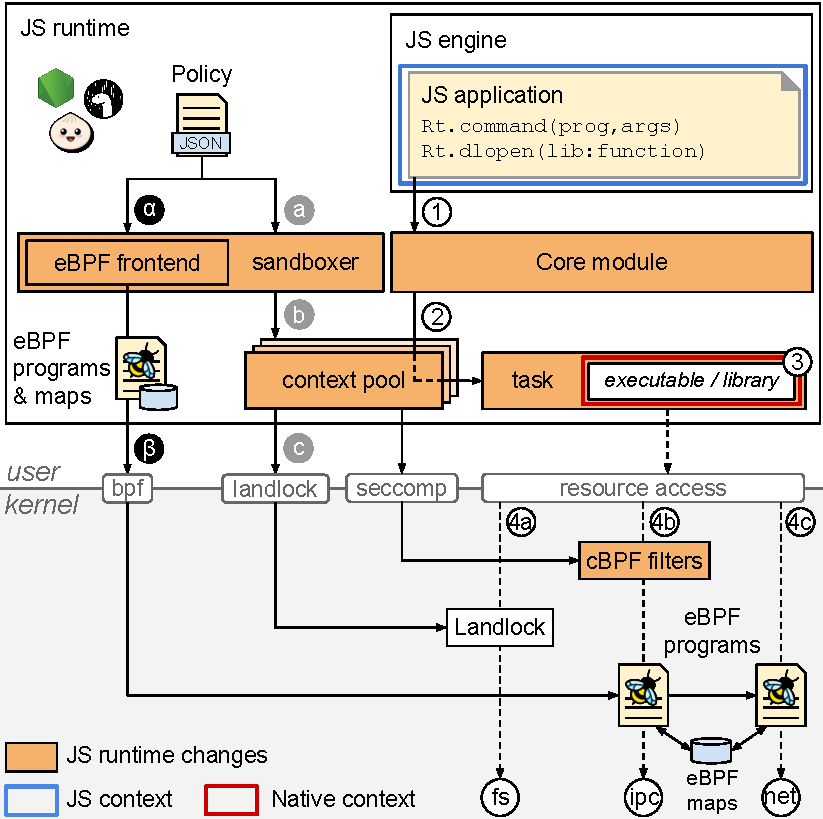
\includegraphics[width=\columnwidth]{chapters/natisand/fig/overview_sandbox}
  \caption[Integration of \natisand in JS runtimes]{
    Integration of \natisand in the JS runtime. Bootstrap: import
    security contexts ($\alpha$,~$\beta$), creation of the context
    pool ($a$,~$b$,~$c$). Application runtime: isolated execution of
    binary programs and shared library functions
    ($1$,~$2$,~$3$,~$4a$,~$4b$,~$4c$)
  }
  \label{fig:overview_sandbox}
\end{figure}
      
The architecture of our solution is shown in
Figure~\ref{fig:overview_sandbox}. Shortly after the JS runtime is
executed, \natisand parses the policy file input by the developer. Based on
the policy, a set of sandboxing and tracing programs
%
along with maps
%
are initialized and loaded into the kernel. A pool of isolated
contexts is also prepared by the sandbox. At runtime, \natisand intercepts
all the calls to native code performed by the application and executes
them safely in the proper isolated context.
%
A technical description of how our proposal is integrated into a
modern JS runtime is given in Section~\ref{subsect:arch}, while
details about its isolation features are reported in
Section~\ref{subsect:isolation}. The policy syntax used by \natisand to
configure permissions, along with the support to policy
generation, are described in Section~\ref{natisand:sect:policy}.


\subsection{Integration with JS runtimes}
\label{subsect:arch}

\natisand complements the architecture of the JS runtime with the addition
of the {\em sandboxer}, a component that parses the policy and
enforces the isolation of native code accordingly. In the following we
explain the operations performed by the runtime to use it, referring to Figure~\ref{fig:overview_sandbox}.

\paragraph{Bootstrap}
The JS runtime boot procedure is modified to read the JSON policy
file, which is then parsed by the sandboxer~\blackcircle{$\alpha$} to
retrieve the information associated with each security context. Based
on the policy,
%
  %
  the sandboxer (i) configures the required Seccomp filters, and (ii)
  prepares and loads into the kernel the necessary eBPF programs and
  maps~\blackcircle{$\beta$}. The eBPF programs are used to track the
  security contexts and enforce network-related and (part of)
  IPC-related restrictions (more details in
  Section~\ref{subsect:isolation}). Maps instead associate each
  isolated compartment with a security policy, and store the ambient
  rights granted to them. To determine which policy is associated with
  a given isolated compartment we leverage its kernel {\tt
    task\textunderscore struct} identifier, which is used as the key
  in an eBPF map of type {\tt TASK\textunderscore STORAGE} to lookup
  the policy identifier. This information is used as an address within
  an eBPF map of type {\tt ARRAY\textunderscore OF\textunderscore
    MAPS}, and permits to retrieve an inner {\tt HASH} map containing
  the ambient rights.
%
Loading eBPF maps and programs is a privileged operation
that requires the {\tt CAP\_BPF}, {\tt CAP\_PERFMON}, {\tt
  CAP\_NET\_ADMIN} capabilities to be performed, thus we grant the JS
runtime executable the corresponding Linux file
capabilities~\cite{file-based-capabilities}.  After the completion of
these steps, the capabilities are no longer necessary, hence they are
dropped. This satisfies the requirement that root permissions at
runtime are not needed for the activation of security contexts.

The sandboxer is also responsible for the creation of the security
contexts where native code will be executed at runtime. Each context
is an OS thread with permissions restricted by Landlock, Seccomp, and
eBPF. To avoid paying the performance cost to instantiate
each security context during the invocation of executables
and shared libraries, we modified the JS runtime to allocate
a thread per security context defined by the policy, restrict their
permissions, and then, park them in a context pool (\graycircle{a},
\graycircle{b}, \graycircle{c}).
%
  %
  With Landlock and Seccomp, restriction of privileges is performed
  calling the corresponding syscalls from the specific context, while
  restriction of permissions based on eBPF is simply performed
  invoking the uprobe {\tt attach\textunderscore policy} reported in
  Table~\ref{table:hooks}a. As a result, the {\tt task\textunderscore
    struct} identifier of a given context is annotated in the
  dedicated eBPF map along with the associated policy identifier.  
%
This design choice allows to reuse security contexts, thus
  minimizing latency, which, as highlighted in the objectives
(Section~\ref{subsect:objectives}), is a critical metric for web
applications.

\paragraph{Application runtime}
After the web application is started, two operations can lead to the
execution of native code: (i) the execution of a binary program in a
subprocess, and (ii) the invocation of a shared library. \natisand
intercepts all the requests originating from the web application that
require to execute native code~\whitecircle{1}, and leverages the
sandboxer to assign them to the proper pre-allocated isolated
context~\whitecircle{2}. Based on the type of request, a dedicated
task inheriting the selected security context is launched and
used to execute the native code~\whitecircle{3}.
Specifically, when there is a request to run an executable,
the JS runtime forks a process. On the other hand, when a shared
library should be loaded, a thread is spawned. The consequence is
that any request to access filesystem, IPC, and network resources will
be subject to the restrictions imposed by the LSMs
(\whitecircle{4a},~\whitecircle{4b},~\whitecircle{4c}). The approach
implemented by \natisand ensures that native code is never loaded nor
executed in a task running unconstrained, thus strengthening the
boundary between the web application and the OS.

\subsection{Isolation features}
\label{subsect:isolation}

Native code executed in isolated contexts can vary from library
functions to entire programs. In the following we detail how \natisand
enforces isolation and summarize the sandboxing features.

\paragraph{Policy inheritance}
While Landlock and Seccomp guarantee policy inheritance after a {\tt
  clone} syscall is performed, the eBPF map that tracks the
restricted contexts must be updated explicitly. To this end, \natisand
relies on the eBPF tracing programs that are loaded into the
kernel during the bootstrap phase and are attached to the {\tt fork}
and {\tt exit} tracepoints reported in
Table~\ref{table:hooks}a. Whenever a security context allocates a new
task with a fork operation, the tracing program registers
a new entry into the map of restricted contexts. The entry
  maps the task identifier of the child to the policy identifier
  associated with the parent. When instead a context terminates its
  duties and issues an exit, its task identifier is deleted from the
  map. No intervention by the developer is required, as policy
inheritance is transparently handled by our solution.

\paragraph{Filesystem}
\natisand restricts access to the filesystem using Landlock. The sandbox
enforces a straightforward {\tt read}, {\tt write}, {\tt exec} (RWX)
permission model, specified with three allow-list vectors (e.g., lines
5, 6, and 7 in Listing~\ref{natisand:lst:policy_file}). After the security
context has been activated, the available permissions can only be
further restricted.

\begin{table}[!t]
	\small
	\begin{tabular}{cc}
	  \parbox{0.47\columnwidth}{
      \centering
      \begin{tabular}{l}
        \toprule
        \multicolumn{1}{c}{\bf Context lifecycle} \\ \midrule
        {\tt uprobe\slash attach\textunderscore policy} \\
        {\tt tp\textunderscore btf\slash sched\textunderscore process\textunderscore fork} \\
        {\tt tp\textunderscore btf\slash sched\textunderscore process\textunderscore exit} \\
        \bottomrule
      \end{tabular}
	  } &
	  \parbox{0.47\columnwidth}{
      \centering
      \begin{tabular}{l | l}
        \toprule
        \multicolumn{2}{c}{\bf Access control}                  \\ \midrule
        \multirow{3}{*}{\rotatebox{90}{IPC}}      & {\tt fentry\slash fifo\_open}     \\
                                  & {\tt lsm\slash socket\_bind}      \\
                                  & {\tt lsm\slash socket\_connect}   \\ \midrule
        \multirow{3}{*}{\rotatebox{90}{Network}}  & {\tt lsm\slash socket\_bind}      \\
                                  & {\tt lsm\slash socket\_create}    \\
                                  & {\tt lsm\slash socket\_connect}   \\
        \bottomrule
      \end{tabular}
	  } \\
	  {\small\bf (a)} & {\small\bf (b)}
	\end{tabular}
	\caption{\label{table:hooks} Hooks and tracepoints monitored by
	  \natisand}
      \end{table}

\paragraph{IPC}
To explain the isolation features \natisand provides, we start with a
description of how programs and libraries generally use IPC.
Native programs often rely on parallelism and concurrency to achieve
high resource utilization. Parallel execution typically requires to
handle synchronization and communication between a parent and a group
of child tasks. In this setting, best practice suggests to provide the
children with the necessary communication channels through the
inheritance properties of the {\tt clone} syscall~\cite{doc-pipe}. For
instance, when two programs are piped in the Bash shell, an IPC
mechanism, in the form of a pipe, is created by the shell process and
is inherited by the two child programs, so that the latter can read
the output from the former. Similarly, a parent and a child task can
leverage an unnamed UNIX socket pair to share
messages~\cite{doc-socketpair}. These use cases do not pose a
significant security risk, since (i) the communication happens between
tasks associated with the same security context, and (ii) the IPC
channels used to communicate are not visible to other services running
on the host OS. Conversely, CVE-2020-16125 and CVE-2021-3560
demonstrate that uncontrolled interaction with globally available IPC
channels used by other services can lead to concrete security
problems.

To block the communication between components associated with
incompatible security contexts, \natisand by default denies IPC over
globally visible communication mechanisms. In this category there are
fifo (i.e., named pipes), message queues, named semaphores,
non-private shared memory, signals, and UNIX named sockets.  Many of
these mechanisms can be fully blocked by denying access to the related
system calls, but in some cases the evaluation of syscall
configuration flags is necessary. For instance, the creation of shared
memory maps is permitted by the sandbox only when the {\tt mmap}
syscall is invoked with {\tt MAP\_ANONYMOUS} or {\tt
  MAP\_PRIVATE}. Similarly, the creation of named special files is
allowed only when the {\tt mknod} and {\tt mknodat} syscalls are not
invoked with {\tt S\_IFIFO} and {\tt S\_IFSOCK}. Syscall filtering
based on configuration flags is performed efficiently by \natisand using
Seccomp.
However, the information available to Seccomp is not always sufficient
to make the access decision. This is the case for the {\tt bind}, {\tt
  connect}, {\tt open}, and {\tt openat} syscalls.  Indeed,
information about the type of socket referenced for the {\tt bind} and
{\tt connect} syscalls resides in user memory, and unfortunately
Seccomp cannot safely dereference it (due to
TOCTOU risks~\cite{seccomp-toctou}). Likewise, the {\tt open} and {\tt openat} syscalls do
not represent the type of file to be opened through configuration
flags, so Seccomp cannot handle the specific case properly. To solve
these problems \natisand relies on the eBPF programs attached to the hooks
reported in Table~\ref{table:hooks}b (which are not affected by TOCTOU
issues, since they operate on arguments that were previously deep
  copied by the kernel). In particular, in the case of UNIX sockets the programs are
attached to the {\tt lsm/socket\_bind} and {\tt lsm/socket\_connect}
hooks, while for fifo files the kernel function {\tt fifo\_open} is
used. A summary of the IPC mechanisms controlled by \natisand, along with
the LSMs leveraged to perform the security checks, is reported in
Table~\ref{table:ipc}.

\paragraph{Network}
%
\natisand permits to control how each isolated context connects to network
resources. In detail, it permits to completely revoke access to the
network, to connect only to a restricted list of hosts, and when
needed, to use the network without restrictions. The sandboxer relies
on eBPF programs to enforce permissions. The programs restrict the
ability to {\tt create}, {\tt connect}, and {\tt bind} sockets, and
are thereby attached to the LSM hooks reported in
Table~\ref{table:hooks}b.

The creation of a socket opens a communication channel and returns a
file descriptor as a result. By default, the sandboxer restricts the
available communication domains to Internet Protocol (IP), denying
applications the use of protocol families such as Bluetooth, Radio,
VSOCK, and many more (this information is directly available
  from the arguments input to the {\tt socket\textunderscore create}
  interface). No restrictions are instead applied to UNIX domain
sockets and the type of socket to be opened (e.g., stream,
datagram). Opening a connection to a host is permitted only when the
developer grants the isolated context to do so. The eBPF
program that checks the opening of a connection first
  recovers the policy restricting the current security context, then
  uses it as a key to lookup the map of ambient rights from the {\tt
    ARRAY\textunderscore OF\textunderscore MAPS} described in
  Section~\ref{subsect:arch}. The ambient rights map is an allow-list
  that stores the reachable (i.e., policy allowed) hosts, hence the
  security check is carried out with a lookup. Each network resource
is uniquely identified by its IP address and port. Internally,
we use the value zero for the port to represent the
  permission of opening a connection to a given host on every port.

Up to now, we have discussed the restrictions when
the application connects as a client to a service. However, web
applications frequently need to serve incoming requests. To do so, it
is necessary to assign a ``name'' to a socket -- i.e., configuring its
address. This operation is done with the {\tt bind} syscall,
  and we decided to permit it only when the policy 
  gives the current security context access to the corresponding
address and port pair. Again, the value zero for the port is used as a
placeholder to allow binding on every port. On the other hand, no
restrictions are applied to the {\tt listen} and {\tt accept}
syscalls. Listen only marks a socket as passive, meaning that it will
be used to accept incoming requests. However, no connection to a
socket can happen if an address was not previously assigned to
it~\cite{doc-listen}.  The same applies to {\tt accept}, which is used
to extract the first connection request from the queue of pending
connections~\cite{doc-accept}.

\begin{table}[t!]
\centering
\small	
\setlength{\tabcolsep}{0.06cm}
\begin{tabular}{| l | l | l | c | c |}
  \hline
  {\bf IPC} & {\bf Subclass} & {\bf Linux system call} & {\bf Seccomp} & {\bf eBPF} \\ \hline
  \multirow{3}{*}{\shortstack[l]{Message \\ queue}}  & \multirow{2}{*}{POSIX}     & mq\_open, mq\_getsetattr, mq\_notify,     & \multirow{2}{*}{\cmark} & \\
            &                            & mq\_timedreceive, mq\_timedsend, mq\_unlink           &                         & \\ \cline{2-5}
            & System V                   & msgctl, msgget, msgrcv, msgsnd            & \cmark                  & \\ \hline
  Pipe      & Named                      & mknod, mknodat, open, openat              & \hspace{0.1cm}\cmark*                 & \cmark \\ \hline
  \multirow{2}{*}{Semaphore}                         & POSIX                      & futex, mmap                               & \hspace{0.1cm}\cmark*                 & \\ \cline{2-5}
            & System V	& semctl, semget, semop, semtimedop         & \cmark                  & \\ \hline
  \multirow{2}{*}{\shortstack[l]{Shared \\ memory}}  & POSIX                      & mmap                                      & \hspace{0.1cm}\cmark*                 & \\ \cline{2-5}
            & System V                   & shmat, shmctl, shmdt, shmget              & \cmark                  & \\ \hline
  \multirow{2}{*}{Signal}                            & Standard  & kill, pidfd\_send\_signal, tgkill, tkill  & \cmark                  & \\ \cline{2-5}
            & Real-time & rt\_sigqueueinfo, rt\_tgsigqueueinfo      & \cmark                  & \\ \hline
  UNIX socket    & Named                      & bind, connect, mknod, mknodat             & \cmark*                 & \cmark \\ \hline
\end{tabular}
\caption[LSMs used by \natisand to restrict Linux IPC]{
  LSMs used by \natisand to restrict Linux IPC. The checkmark
  \cmark* indicates when Seccomp needs to evaluate the syscall
  configuration flags to make the access decision
}
\label{table:ipc}
\end{table}

  \paragraph{Limitations}
  %
  While \natisand significantly restricts the set of permissions and system
  resources associated with subprocesses and shared libraries, it
  provides strong memory isolation guarantees only when executables
  are run, as each subprocess is executed within its own address
  space. On the other hand, shared libraries are loaded within the
  hosting thread address space, hence a native library bug can impact
  the web application memory. Several research works have studied this
  problem and have proposed countermeasures~\cite{RLBox,
    kirth2022pkru, wu2012codejail, cali, vasilakis2018breakapp,
    binwrap}. In general, these works are compatible with the design
  of our solution, therefore they could be used in conjuction with
  \natisand to improve isolation of shared libraries. Among them,
  BreakApp~\cite{vasilakis2018breakapp} and BinWrap~\cite{binwrap}
  propose approaches tailored for interpreted languages, but they
  require either the introduction of wrappers or the execution of
  remote procedure calls. RLBox~\cite{RLBox} provides strong
  guarantees against memory corruption, but it demands the developer
  to manually retrofit existing code, a process that can take up to
  ``few days'' for each library according to the authors. Improved
  intra-process isolation can also be achieved leveraging dedicated
  hardware features like Intel Protection Keys for Userspace (PKU),
  but as demonstrated by PKU Pitfalls~\cite{pku-pitfalls} these
  solutions can be bypassed using kernel functions that are agnostic
  of intra-process isolation (i.e., the attacks use the kernel as a
  confused deputy). Since \natisand is completely aligned with the memory
  isolation assumptions made by the kernel, our solution is not
  affected by this issue.  




%%% Local Variables:
%%% mode: latex
%%% TeX-master: "../main.tex"
%%% End:
